\documentclass[../main.tex]{subfiles}

\begin{document}

%%%%%%%%%%%%%%%%%%%%%%%%%%%%%%%%%%%%%%%%%%%%%%%%%%%%%%%%%%%%%%%%%%%%%%%%%%%%%%%%%%%%%

\section{Uge 2 -- Ækvivalensprincippet}
\setcounter{section}{2}


%%%%%%%%%%%%%%%%%%%%%%%%%%%%%%%%%%%%%%%%%%%%%%%%%%%%%%%%%%%%%%%%%%%%%%%%%%%%%%%%

\subsection{Opgave 1 -- Observatør i inertialsystem og ikke-inertialsystem}
\setcounter{subsection}{1}
\setcounter{equation}{0}

Et pendul hænger ned fra taget inde i en bil, som bevæger sig i en lige linje med konstant acceleration $a$. Find vinklen som pendulet har til vertikal. Forklar hvad der sker for en inertial observatør placeret udenfor bilen og en ikke-inertial observatør i bilen.

%%%%%%%%%%%%%%%%%%%%%%%%%

\subsubsection{Besvarelse}

\ldots



%%%%%%%%%%%%%%%%%%%%%%%%%%%%%%%%%%%%%%%%%%%%%%%%%%%%%%%%%%%%%%%%%%%%%%%%%%%%%%%%

\subsection{Opgave 2 -- Spand med vand på skråplan}
\setcounter{subsection}{2}
\setcounter{equation}{0}

En spand med vand glider grundet tyngdekraft ned af et skråplan i en fikseret vinkel $\alpha$ til horisontal uden friktion. Hvad er vinklen for hældningen af vandet relativt til spandens bund?

%%%%%%%%%%%%%%%%%%%%%%%%%

\subsubsection*{Besvarelse}

Fra geometri vides det, at de to overforstående vikler, som danner af to linjer, der mødes, er ens. Bruger vi dette samt at kunne forskyde trekanter, da får vi
\begin{center}
    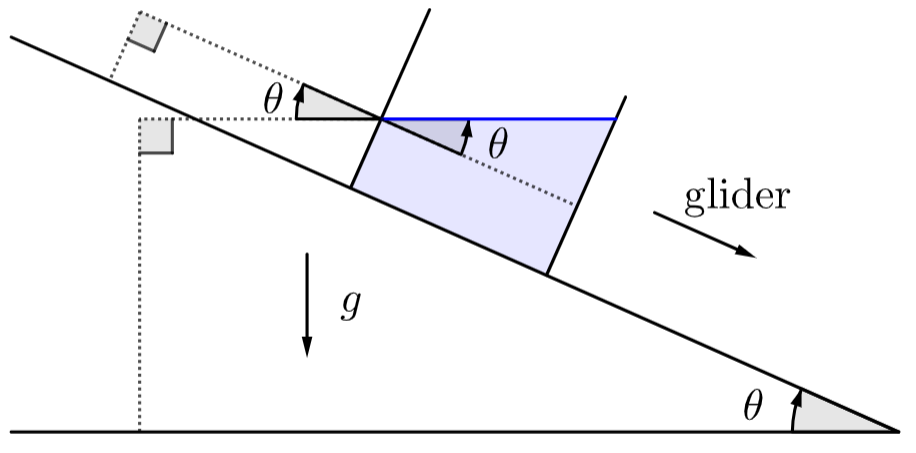
\includegraphics[width=.75\textwidth]{../billeder/BucketOnInclinedPlane.PNG}
\end{center}



%%%%%%%%%%%%%%%%%%%%%%%%%%%%%%%%%%%%%%%%%%%%%%%%%%%%%%%%%%%%%%%%%%%%%%%%%%%%%%%%

\subsection{Opgave 3 -- Newtonsk tyngdekraft}
\setcounter{subsection}{3}
\setcounter{equation}{0}

\paragraph{a)} Argumentér for at bevægelsesligningerne for et testobjekt med koordinat $\vv{r}$ i Newtons teori om tyngdekraft,
\begin{align} \label{eq:Uge2_Opg3_NewtonsEquationOfMotion}
    \ddt{\vv{r}} &= - \sum_k \frac{G_N M_k}{\abs{\vv{r} - \vv{r}_k}^2} \frac{\vv{r} - \vv{r}_k}{\abs{\vv{r} - \vv{r}_k}} \: ,
\end{align}
hvor $M_k$ og $\vv{r}_k$ er massen og koordinatet for tyngdekraftudøvende objekter, kan skrives som
\begin{align}
    \ddt{\vv{r}} &= - \Grad{\phi} \: ,
\end{align}
hvor $\phi$ er det gravitationelle potential,
\begin{align}
    \phi(\vv{r}) &= - \sum_k \frac{G_N M_k}{\abs{\vv{r} - \vv{r}_k}} \: .
\end{align}

\paragraph{b)} Argumentér for at det gravitationelle potential opfylder ligningen
\begin{align} \label{eq:Uge2_Opg3_LaplaceOfGravitationalPotential}
    \laplace{\phi(\vv{r})} &= 4 \pi G_N \mu(\vv{r})
\end{align}
hvor $\mu(\vv{r})$ er densiteten af masse af de tyngdekraftudøvende objekter,
\begin{align}
    \mu(\vv{r}) &= \sum_k M_k \delta^3(\vv{r} - \vv{r}_k) \: .
\end{align}
Hint: $\laplace{\inv{r}} = - 4\pi\delta^3(\vv{r})$ \cite[ligning 1.102]{Griffiths_eldyn}.

\paragraph{c)} Argumentér for at \cref{eq:Uge2_Opg3_NewtonsEquationOfMotion,eq:Uge2_Opg3_LaplaceOfGravitationalPotential} er invariante under Galilæitransformationen.

%%%%%%%%%%%%%%%%%%%%%%%%%

\subsubsection*{Besvarelse}

%%%%%%%%%%%%%%%%%%%%%%%%%

\paragraph{a)}

Til dette indsættes udtrykket for $\phi$ i ligningen for $\ddt{\vv{r}}$, hvilket giver
\begin{align}
\begin{split}
    \ddt{\vv{r}} &= - \Grad{\phi(\vv{r})} \\
        &= - \Grad{\left( - \sum_k \frac{G_N M_k}{\abs{\vv{r} - \vv{r}_k}} \right)} \\
        &= \sum_k G_N M_k \Grad{\left( \inv{\abs{\vv{r} - \vv{r}_k}} \right)} \\
        &= \sum_k G_N M_k \frac{- \left( \vv{r} - \vv{r}_k \right)}{\abs{\vv{r} - \vv{r}_k}^3} \\
        &= - \sum_k \frac{G_N M_k}{\abs{\vv{r} - \vv{r}_k}^2} \frac{\vv{r} - \vv{r}_k}{\abs{\vv{r} - \vv{r}_k}}
\end{split}
\end{align}
hvor vi har benyttet, at
\begin{align}
    \Grad{\left(\inv{r'}\right)} &= - \frac{\rhat'}{r'^2}
        = - \frac{\vv{r}'}{r'^3} \: ,
\end{align}
da $\rhat' = \vv{r}' / r'$.
Dermed har vi vist bevægelsesligningen, \cref{eq:Uge2_Opg3_NewtonsEquationOfMotion}, som vi skulle finde.


%%%%%%%%%%%%%%%%%%%%%%%%%

\paragraph{b)}

Dette kan vises ved brug af Greensfunktionen (\cite[ligning 1.102]{Griffiths_eldyn})
\begin{align}
    \laplace{\inv{r}} = - 4\pi\delta^3(\vv{r}) \: ,
\end{align}
hvormed vi får, at
\begin{align}
\begin{split}
    \laplace{\phi(\vv{r})} &= \laplace{\left( - \sum_k \frac{G_N M_k}{\abs{\vv{r} - \vv{r}_k}} \right)} \\
        &= - \sum_k G_N M_k \laplace{\left( \inv{\abs{\vv{r} - \vv{r}_k}} \right)} \\
        &= - \sum_k G_N M_k \left[ - 4\pi \delta^3(\vv{r} - \vv{r}_k) \right] \\
        &= 4 \pi G_N \sum_k M_k \delta^3(\vv{r} - \vv{r}_k) \\
        &= 4 \pi G_N \mu(\vv{r}) \: ,
\end{split}
\end{align}
hvor $\mu(\vv{r})$ er densiteten af masse af de tyngdekraftudøvende objekter,
\begin{align}
    \mu(\vv{r}) &= \sum_k M_k \delta^3(\vv{r} - \vv{r}_k) \: .
\end{align}
Dette er præcis \cref{eq:Uge2_Opg3_LaplaceOfGravitationalPotential}, som skulle vises.


%%%%%%%%%%%%%%%%%%%%%%%%%

\paragraph{c)}

Det skal nu argumenteres for, at \cref{eq:Uge2_Opg3_NewtonsEquationOfMotion,eq:Uge2_Opg3_LaplaceOfGravitationalPotential} er invariante under Galilæitransformationen.

Galilæitransformationen lyder $t' = t$ og $\vv{r}' = \vv{r} - \vv{v} t$. For at finde de to ligninger differentierer vi $\phi(\vv{r})$ med hensyn til $\vv{r}$, hvorfor ledet $- \vv{v} t$ forsvinder for både $\ddt{\vv{r}}$ og $\laplace{\phi(\vv{r})}$. Derved er dette svarende til, at transformation havde lydt $t' = t$ og $\vv{r}' = \vv{r}$, hvormed det trivielt ses, at \cref{eq:Uge2_Opg3_NewtonsEquationOfMotion,eq:Uge2_Opg3_LaplaceOfGravitationalPotential} er invariante under.



%%%%%%%%%%%%%%%%%%%%%%%%%%%%%%%%%%%%%%%%%%%%%%%%%%%%%%%%%%%%%%%%%%%%%%%%%%%%%%%%

\subsection{Opgave 4 -- Tyngdekraft som geometri af rummet}
\setcounter{subsection}{4}
\setcounter{equation}{0}

\paragraph{a)} Argumentér for at den ikke-relativistiske bevægelse af et testobjekt med masse $m$ i et Newtonsk gravitationelt potential $\phi$ kan beskrives ved Lagrangefunktionen
\begin{align} \label{eq:Uge2_Opg4_Lagrangian}
    L &= \inv{2} m \vv{v}^2 - m \phi - m c^2 \: ,
\end{align}
hvor $v$ er hastigheden af objektet.

\paragraph{b)} Argumentér for at denne Lagrangefunktion kan opnås som den ikke-relativistiske grænse med svagt felt ($v \ll c$ og $\phi \ll c^2$) fra virkningen $S = - mc \int \dd s$, hvor det infinitesimale interval $\dd s$ er givet som
\begin{align}
    \dd s^2 &= \left( 1 + \frac{2\phi}{c^2} \right) c^2 \dd t^2 - \dd \vv{r}^2 \: .
\end{align}

\paragraph{c)} Argumentér for at denne metrik beskriver et kurvet (ikke-Euklidisk) rum og at egentiden (eng: proper time) løber forskelligt i forskellige højder i det gravitationelle potential.


%%%%%%%%%%%%%%%%%%%%%%%%%

\subsubsection*{Besvarelse}

%%%%%%%%%%%%%%%%%%%%%%%%%

\paragraph{a)}

For en partikel i et konservativt felt, som tyngdefeltet, er den generelle Lagrangefunktion
\begin{align} \label{eq:Uge2_Opg4_LagrangianGeneral_L=T+V}
    L &= T - V \: ,
\end{align}
hvor $T$ er partiklens kinetiske energi og $V(\vv{r})$ dens potentielle energi associeret med det konservative felt.
For vores partikel er den kinetiske energi blot
\begin{align}
    T &= \frac{m\vv{v}^2}{2} - m c^2 \: ,
\end{align}
hvor $mv^2/2$ er fra den generelle bevægelse af partiklen og $mc^2$ fra \ldots. Den potentielle energi for partiklen med masse $m$ i tyngdefeltet er
\begin{align}
    V(\vv{r}) &= m \phi(\vv{r}) \: .
\end{align}
Indsættes disse to udtryk i det generelle udtryk for Lagrangefunktionen, \cref{eq:Uge2_Opg4_LagrangianGeneral_L=T+V}, findes
\begin{align}
    L &= \inv{2} m \vv{v}^2 - m \phi - m c^2 \: ,
\end{align}
hvilket var Lagrangefunktionen, som skulle findes.

%%%%%%%%%%%%%%%%%%%%%%%%%

\paragraph{b)}

Vi betragter virkningen
\begin{align} \label{eq:Uge2_Opg4_LagrangianFromActionCalculation_Part1}
\begin{split}
    S &= - mc \int \dd s \\
        &= - mc \int \left[ \left( 1 + \frac{2\phi}{c^2} \right) c^2 \dd t^2 - \dd \vv{r}^2 \right]^{1/2} \\
        &= - mc \int \left[ \left( 1 + \frac{2\phi}{c^2} \right) c^2 - \vv{v}^2 \right]^{1/2} \dd t \\
        &= - mc^2 \int \left[ \left( 1 + \frac{2\phi}{c^2} \right) - \frac{\vv{v}^2}{c^2} \right]^{1/2} \dd t \: ,
\end{split}
\end{align}
hvor vi først har trukket $\dd t$ udenfor og brugt at $\vv{v} = \dd \vv{r} / \dd t$, hvorefter en faktor $c$ er blevet trukket udenfor.

Idet at $v \ll c$ og $\phi \ll c^2$ kan vi Taylorudvikle \cref{eq:Uge2_Opg4_LagrangianFromActionCalculation_Part1} til første orden omkring $0$, hvilket giver
\begin{align}
    S &\simeq - mc^2 \int \left( \sqrt{1 - \frac{\vv{v}^2}{c^2}} - \frac{2\frac{\phi}{c^2}}{\sqrt{1 - \frac{\vv{v}^2}{c^2}}} \right) \dd t \: .
\end{align}
Udvikler vi nu kvadratrødderne til første orden, da vi stadig er i grænsen beskrevet ovenfor, fås
\begin{align}
    \sqrt{1 + x} \simeq 1 - \inv{2} x \: ,
        \quad \text{og} \quad
    \sqf{1}{1 + x} \simeq 1 + \inv{2} x \: ,
\end{align}
da $[1 + x]^n \simeq 1 - nx$ for $x \ll 1$, hvormed virkningen bliver
\begin{align}
\begin{split}
    S &\simeq - mc^2 \int \left( 1 - \frac{\vv{v}^2}{2c^2} - \frac{\phi}{c^2} \left[ 1 - \frac{\vv{v}^2}{c^2} \right] \right) \dd t \\
        &\simeq - mc^2 \int \left( 1 - \frac{\vv{v}^2}{2c^2} - \frac{\phi}{c^2} \right) \dd t \\
        &= \int \left( -m c^2 + \frac{m \vv{v}^2}{2} + m \phi \right) \dd t
\end{split}
\end{align}
hvor vi har negligeret faktoren $\phi \vv{v}^2 / c^4$.

Siden $S = \int L\, \dd t$ må
\begin{align}
    L &= \inv{2} m \vv{v}^2 - m \phi - m c^2 \: .
\end{align}
Dermed er det vist, at Lagrangefunktionen, \cref{eq:Uge2_Opg4_Lagrangian}, kan findes fra virkningen i grænsen hvor $v \ll c$ og $\phi \ll c^2$.


%%%%%%%%%%%%%%%%%%%%%%%%%

\paragraph{c)}

Da rumtiden i et gravitationelt potential kun lokalt og ikke globalt kan transformeres til en (fladt) Minkowskirumtid, så giver det mening, at metrikken kaldes ''kurvet'', ''krum'' eller ''ikke-Euklidisk'', da vi ikke kan have globale flade koordinater, hvorfor de nogle steder må være ikke-flade. Dette skyldes generelt at tiden er afhængig af en faktor, som afhænger af det gravitationelle potential, hvilket vises herunder.
\\

Opgavens metrik er
\begin{align}
    \dd s^2 &= \left( 1 + \frac{2\phi}{c^2} \right) c^2 \dd t^2 - \dd \vv{r}^2 \: ,
\end{align}
og sammenlignes denne med Minkowskimetrikken,
\begin{align}
    \dd s^2 &= c^2 \dd t^2 - \dd \vv{r}^2 \: ,
\end{align}
så ses det, at frontfaktoren for  $00$-komponenten er ændret. Dermed må der også være den samme ændring for egentiden, så egentiden målt af en observatør i opgavens metrik er
\begin{align}
    \dd \tau &= \left( 1 + \frac{2\phi}{c^2} \right) \dd t \: .
\end{align}

Vi betragter nu to observatører, som befinder sig i det gravitationelle potential: Én observatør er i højden $a$ og den anden i højden $b = a + h$, hvor $h$ er højdeforskellen mellem de to observatører. Egentiden målt for disse to observatører bliver
\begin{subequations}
\begin{align}
    \dd \tau_a &= \left( 1 + \frac{2\phi_a}{c^2} \right) \dd t \: , \quad \text{og} \\
    \dd \tau_b &= \left( 1 + \frac{2\phi_b}{c^2} \right) \dd t \: .
\end{align}
\end{subequations}
Siden $\phi_b - \phi_a = \phi(a + h) - \phi(a) = \phi(h)$, da $\phi(x) = gx$, hvor $g$ er tyngdeaccelerationen og $x$ placeringen af partiklen i potentialet, da bliver tidsforskellen mellem disse to observatører
\begin{align}
    \Delta \tau_{ab} &= \frac{2(\phi_b - \phi_a)}{c^2} \dd t
        = \frac{2\phi(h)}{c^2} \dd t \: .
\end{align}
Dermed er det vist, at egentiden målt af observatører i forskellig højde i samme gravitationelle potential er forskellig, altså at egentiden afhænger af, hvor i det gravitationelle potential, som man er.



%%%%%%%%%%%%%%%%%%%%%%%%%%%%%%%%%%%%%%%%%%%%%%%%%%%%%%%%%%%%%%%%%%%%%%%%%%%%%%%%

\subsection{Opgave 5 -- Forklaring af tvillingeparadokset}
\setcounter{subsection}{5}
\setcounter{equation}{0}

Forklar tvillingeparadokset i speciel relativitetsteori set fra
\paragraph{a)} den inertiale tvillings synspunkt, og
\paragraph{b)} den ikke-inertiale (rejsende) tvillings synspunkt.

%%%%%%%%%%%%%%%%%%%%%%%%%

\subsubsection{Besvarelse}

Tvillingeparadoket omhandler et tvillingepar, hvor den ene tvilling bliver tilbage på Jorden mens den anden rejser væk fra Jorden med en betydelig brøkdel af lysets hastighed. Når den rejsenede tvilling kommer tilbage på Jorden, da vil den inertiale tvilling have ældet mere end den rejsende tvilling, da et ur i bevægelse går langsomt.
% Man kan for illustrationens skyld antage, at de to tvillinger ved brug af lys sender hinanden en fødselsdagshilsen hver gang, at de selv ældes ét år.

%%%%%%%%%%%%%%%%%%%%%%%%%

\paragraph{a)}

Set fra den inertiale tvillings synspunkt ses det, at den rejsende tvilling rejser ud i universet, hvorfor dennes ur må bevæge sig langsommere end den inertiale tvillings, da et ur i bevægelse bevæger sig langsommere, og ved den rejsende tvillings hjemkomst vil alderen af den rejsende tvilling, når den inertiale tvillings alder er $t$, være
\begin{align}
    t' &= \frac{t}{\gamma} \: .
\end{align}


%%%%%%%%%%%%%%%%%%%%%%%%%

\paragraph{b)}

''Paradokset'' opstår når man observerer det samme scenarie fra den rejsende tvillings perspektiv. Her ser den rejsende tvilling, at den inertiale tvilling bevæger sig væk, hvorfor det må være den inertiale tvillings ur, som går langsommere, hvorved den rejsende tvilling vil mene, at den inertiale tvilling er yngst ved deres genforening, altså at
\begin{align}
    t &= \frac{t'}{\gamma} \: .
\end{align}

De ''manglende'' år $\Delta t = t_a - t_b = t - t' = t (1 - 1/\gamma^2)$ skyldes, at den rejsende tvilling ikke har medtaget, at personen skifter inertialsystem idet der vendes om for at rejse tilbage til Jorden, hvilket ikke er blevet medtaget i beregningerne. De manglende år kan ses at komme fra princippet om, at hvis man er bagud i bevægelsesretningen, så er man foran i tid. På udturen ser den rejsende tvilling, at den inertiale tvilling bevæger sig væk, hvorfor denne må være forrest i bevægelsesretningen og dermed bagerst i tid (aka. yngre), mens dette billede vendes på hovedet, når der skiftes inertialsystem, da den inertiale tvilling da bevæger sig imod den rejsende tvilling, hvorved den inertiale tvilling er bagerst i bevægelsesretningen, hvorfor dennes ur dermed er foran (aka. ældre). Bruges Lorentztransformationerne ses det, at medtagelsen af inertialsystemsskiftet for den rejsende tvilling i Lorentztransformationerne netop giver $\Delta t$, altså de år som ''manglede''. Dette betyder ikke, at den inertiale tvilling ældes $\Delta t$ år, idet at den rejsende tvilling skifter inertialsystem, men blot at den rejsende tvillings forståelse af, hvor gammel den inertiale tvilling er, skifter med $\Delta t$ år i vendepunktet.

Der er dermed ikke tale om er rigtigt paradoks, da der er en fysisk forklaring på uoverensstemmelsen, men det kan ligne et paradoks.



%%%%%%%%%%%%%%%%%%%%%%%%%%%%%%%%%%%%%%%%%%%%%%%%%%%%%%%%%%%%%%%%%%%%%%%%%%%%%%%%

\subsection{Opgave 6 -- Bevægelse af fri partikel i uniformt gravitationelt felt}
\setcounter{subsection}{6}
\setcounter{equation}{0}

Hvad er bevægelsen (eng: path) af en fri partikel i et uniformt gravitationelt felt?

%%%%%%%%%%%%%%%%%%%%%%%%%

\subsubsection{Besvarelse}

\ldots



%%%%%%%%%%%%%%%%%%%%%%%%%%%%%%%%%%%%%%%%%%%%%%%%%%%%%%%%%%%%%%%%%%%%%%%%%%%%%%%%

\subsection{Opgave 7 -- Afbøjning af lys i gravitationelle felter grundet ækvivalenspricippet}
\setcounter{subsection}{7}
\setcounter{equation}{0}

Argumentér for at ækvivalenspricippet medfører, at lys bliver afbøjet i gravitationelle felter.

%%%%%%%%%%%%%%%%%%%%%%%%%

\subsubsection{Besvarelse}

Ækvivalensprincippet siger, at man lokalt ikke kan se foreskel på tyngdekraft og kraften af en anden acceleration. Sagt med andre ord: Hvis du befinder dig indelukket i en elevator uden vinduer eller andet til at fortælle dig, hvor du befinder dig, så vil du ikke kunne fortælle, om elevatoren befinder sig stillestående på Jorden, hvor den påvirkes med tyngdeaccelerationen, eller om den bevæger sig med acceleration $a = g$ langt fra alle graviterende objekter.

Antager vi nu, at vi befinder os i denne elevator, som bevæger sig i rummet langt fra alle graviterende objekter med konstant acceleration, da vil vi se, at en lyspuls udsendt horisontalt fra elevatorens ene væg vil falde som tiden går, hvilket vises af nedenstående billede.
\begin{center}
    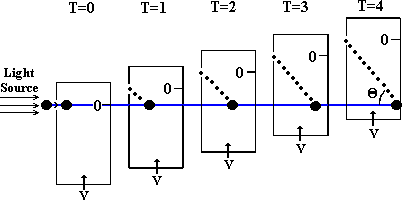
\includegraphics[width=.6\textwidth]{billeder/LightBendingInRocket2.png}
\end{center}
Dette billede er måske lidt misvisende, da det godt nok afbilleder situationen, hvis der havde været konstant hastighed, hvorved lyset ikke ville afbøjes men blot være lineært i en vinkel til horisontal, men det er medtaget for at vise, hvordan vi langs $\xhat$-aksen har tiden. Forestilles i stedet, at vi har konstant acceleration, da vil hastigheden blive større og større, hvorved lyspulsen efter ét tidsskridt vil være faldet mere end efter det foregående tidsskridt, altså er lyspulsen afbøjet. Grundet ækvivalenspricippet må dette medføre, at lys afbøjes i et gravitationelt felt, hvilket kan ses på nedenstående billede.
\begin{center}
    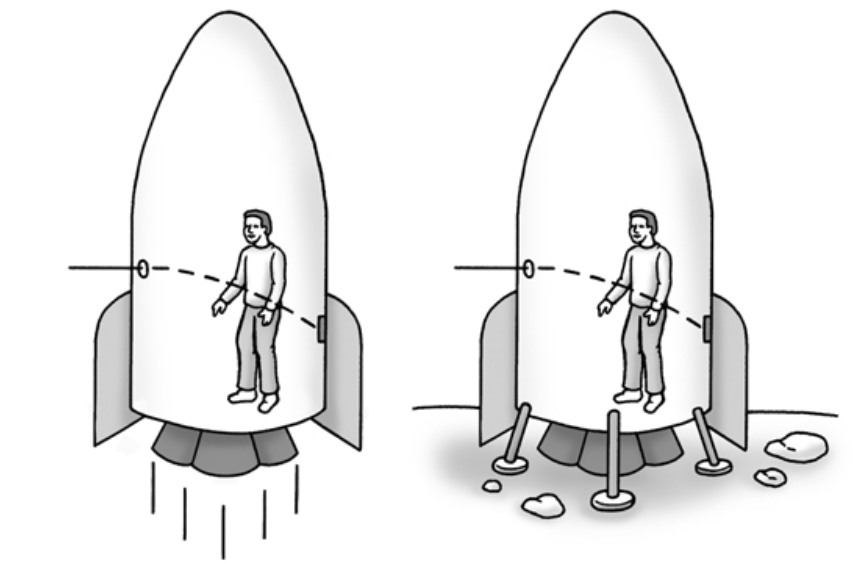
\includegraphics[width=.6\textwidth]{billeder/LightBendingInRocket.PNG}
\end{center}



%%%%%%%%%%%%%%%%%%%%%%%%%%%%%%%%%%%%%%%%%%%%%%%%%%%%%%%%%%%%%%%%%%%%%%%%%%%%%%%%

\subsection{Opgave 8 -- Gravitationel rødforskydning grundet ækvivalenspricippet}
\setcounter{subsection}{8}
\setcounter{equation}{0}

Argumentér for at ækvivalensprincippet medfører gravitationel rødforskydning.

%%%%%%%%%%%%%%%%%%%%%%%%%

\subsubsection{Besvarelse}

Ækvivalensprincippet siger, at man lokalt ikke kan se foreskel på tyngdekraft og kraften af en anden acceleration. Sagt med andre ord: Hvis du befinder dig indelukket i en elevator uden vinduer eller andet til at fortælle dig, hvor du befinder dig, så vil du ikke kunne fortælle, om elevatoren befinder sig stillestående på Jorden, hvor den påvirkes med tyngdeaccelerationen, eller om den bevæger sig med acceleration $a = g$ langt fra alle graviterende objekter.

Antager vi nu, at vi befinder os i denne elevator, som bevæger sig i rummet langt fra alle graviterende objekter med konstant acceleration $a = g$, da vil vi observere, at en lyspuls sendt op fra gulvet i elevatoren mod taget af denne vil være rødforskudt. Dette skyldes, at elevatorens tag også bevæger sig opad, så for at blive målt skal lyspulsen altså indhente elevatorens tag, hvormed afstanden, som lyspulsen har bevæget sig, er blevet længere. De to scenarier -- en lyspuls sendt fra gulv til loft i hhv. en elevator uden ydre påvirkning og en elevator med konstant acceleration -- er afbildet nedenfor.
\begin{center}
    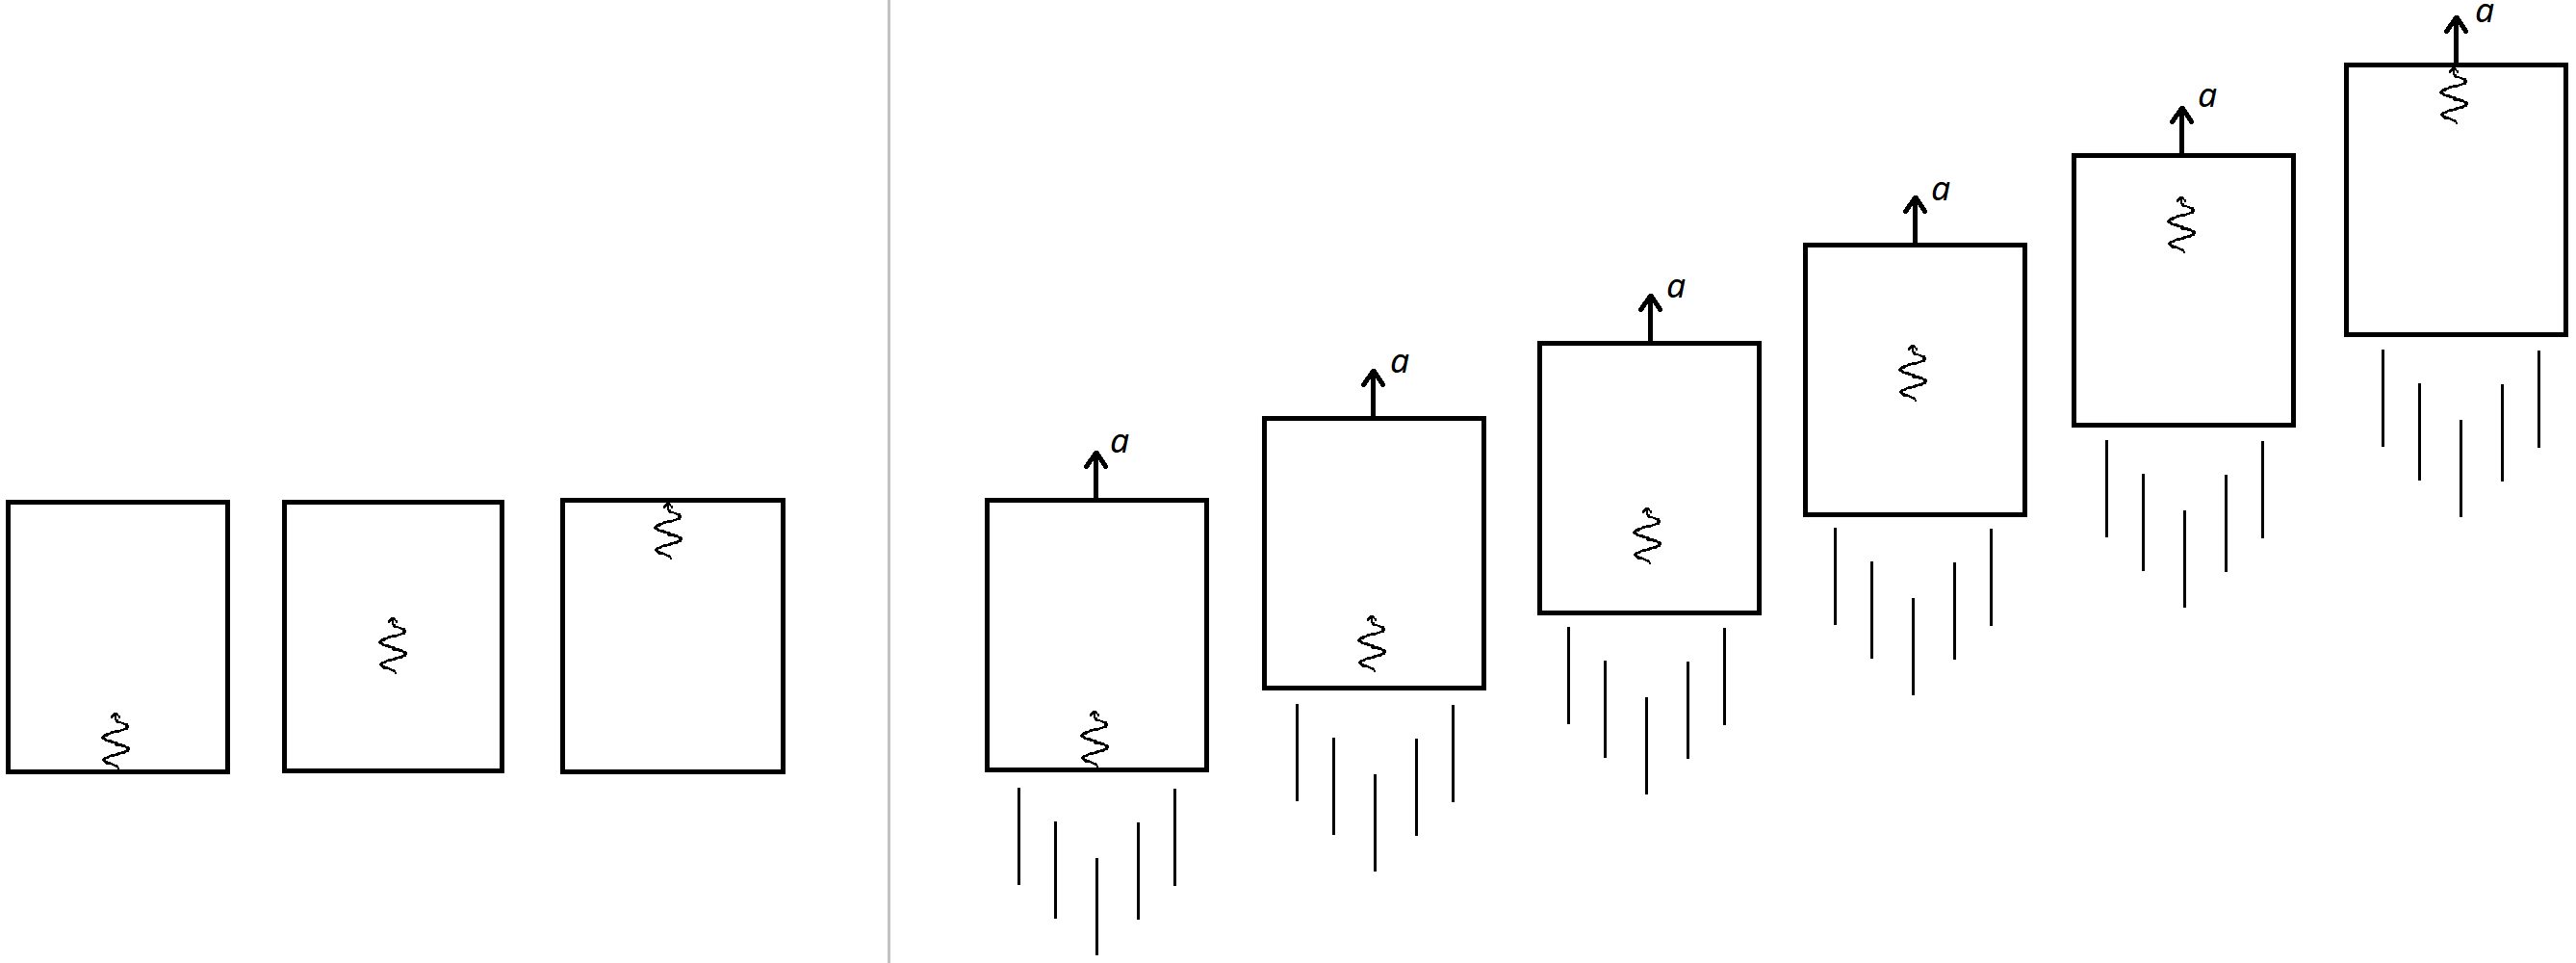
\includegraphics[width=\textwidth]{billeder/GravitationalRedshift.png}
\end{center}
Idet at der sker denne rødforskydning i tilfældet, hvor elevatoren bevæger sig med konstant acceleration, da dikterer ækvivalensprincippet, at den samme rødforskydning må være tilfældet grundet gravitation. Vi kan altså ikke se forskel på en kinematisk rødforskydning og en gravitationel rødforskydning.



%%%%%%%%%%%%%%%%%%%%%%%%%%%%%%%%%%%%%%%%%%%%%%%%%%%%%%%%%%%%%%%%%%%%%%%%%%%%%%%%

\subsection{Opgave 9 -- Er opgave 7 eller opgave 8 i inertialsystem?}
\setcounter{subsection}{9}
\setcounter{equation}{0}

Konstruér et eksperiment til at identificere, hvilket af \textbf{7)} og \textbf{8)} som er i et inertialsystem.

%%%%%%%%%%%%%%%%%%%%%%%%%

\subsubsection{Besvarelse}

\ldots



%%%%%%%%%%%%%%%%%%%%%%%%%%%%%%%%%%%%%%%%%%%%%%%%%%%%%%%%%%%%%%%%%%%%%%%%%%%%%%%%

\subsection{Opgave 10 -- Tilladte koordinattransformationer i GR}
\setcounter{subsection}{10}
\setcounter{equation}{0}

Er de følgende koordinattransformationer $(x,\, y) \rightarrow (x',\, y')$ tilladte i generel relativitetsteori?
\paragraph{a)} $x' = x$, $y' = 1$.
\paragraph{b)} $x' = \sqrt{x^2 + y^2}$, $y' = \arctan(y/x)$.
\paragraph{c)} $x' = 1/\sqrt{x^2 + y^2}$, $y' = \arctan(y/x)$.
\paragraph{d)} $x' = \ln(x)$, $y' = y$.

%%%%%%%%%%%%%%%%%%%%%%%%%

\subsubsection*{Besvarelse}

I generel relativitetsteori er de tilladte koordinattransformationer dem, som er invertible og som har koordinater, der er differentiable.

%%%%%%%%%%%%%%%%%%%%%%%%%

\paragraph{a)}

Ikke tilladt.

Det ses her trivielt, at denne transformation ikke er invertibel, siden der ikke mappes til $y$.


%%%%%%%%%%%%%%%%%%%%%%%%%

\paragraph{b)}

Tilladt.

Det ses trivielt, at begge koordinater er differentiable -- der er tale om kvadratrødder brøker, kvadrater og trigonometriske funktioner -- og det er muligt at invertere transformationen
\begin{subequations}
\begin{align}
    x &= x' \sqf{1}{1 + \tan^2(y')} \: , \quad \text{og} \\
    y &= \frac{\tan(y')x'}{\sqrt{1 + \tan^2(y')}} \: .
\end{align}
\end{subequations}
(Dette beregnes ved substitution, som normalt for $z$ ligninger med $z$ ubekendte.)


%%%%%%%%%%%%%%%%%%%%%%%%%

\paragraph{c)}

Tilladt.

Det ses trivielt, at begge koordinater er differentiable -- der er tale om kvadratrødder brøker, kvadrater og trigonometriske funktioner -- og det er muligt at invertere transformationen
\begin{subequations}
\begin{align}
    x &= \inv{x'}\, \sqf{1}{1 - \tan^2(y')} \: , \quad \text{og} \\
    y &= \frac{\tan(y')}{x'\sqrt{1 - \tan^2(y')}} \: .
\end{align}
\end{subequations}
(Dette beregnes ved substitution, som normalt for $z$ ligninger med $z$ ubekendte.)


%%%%%%%%%%%%%%%%%%%%%%%%%

\paragraph{d)}

Tilladt.

Det ses trivielt, at begge koordinater er differentiable -- der er tale om logaritmer og lineære funktioner -- og det er muligt at invertere transformationen
\begin{subequations}
\begin{align}
    x &= \pexp{x'} \: , \quad \text{og} \\
    y &= y' \: .
\end{align}
\end{subequations}



%%%%%%%%%%%%%%%%%%%%%%%%%%%%%%%%%%%%%%%%%%%%%%%%%%%%%%%%%%%%%%%%%%%%%%%%%%%%%%%%%%%%%

\end{document}